\documentclass[tikz,border=8pt]{standalone}
\usepackage[T1]{fontenc}
\usepackage[utf8]{inputenc}
\usepackage{amsmath}
\usepackage{xcolor}
\usetikzlibrary{arrows.meta,calc,decorations.pathreplacing,positioning}

\definecolor{itblue}{RGB}{40,86,135}
\definecolor{itlightblue}{RGB}{229,239,249}
\definecolor{itgreen}{RGB}{30,128,92}
\definecolor{itlightgreen}{RGB}{226,244,236}
\definecolor{itorange}{RGB}{232,126,32}
\definecolor{itlightorange}{RGB}{255,235,209}
\definecolor{itgray}{RGB}{92,99,112}

\begin{document}
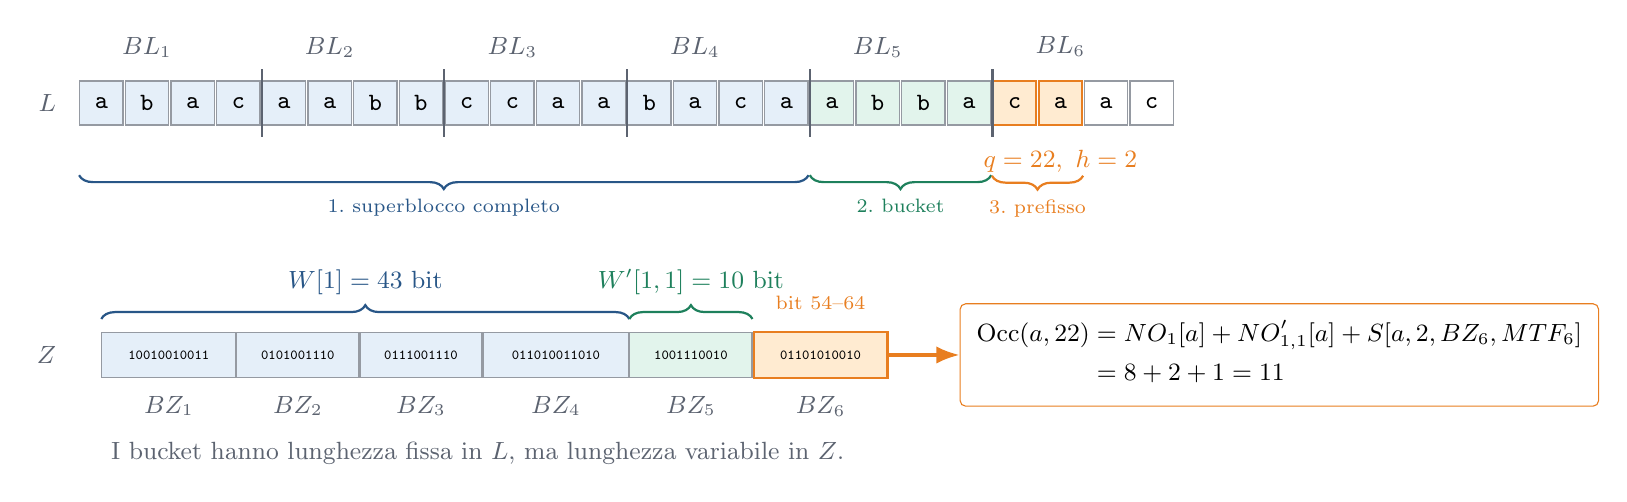
\begin{tikzpicture}[
    >=Latex,
    char/.style={
        draw=itgray!65,
        minimum width=0.55cm,
        minimum height=0.56cm,
        inner sep=0pt,
        font=\small\ttfamily
    },
    bitblock/.style={
        draw=itgray!65,
        minimum height=0.58cm,
        inner sep=3pt,
        font=\tiny\ttfamily
    },
    label/.style={font=\small, text=itgray},
    note/.style={font=\small, align=center},
    arrow/.style={->, very thick, itorange}
]

% Logical partition of L. The toy value ell=4 keeps all three query
% contributions visible in one compact example.
\node[label, anchor=east] at (-0.45,0) {$L$};
\foreach \j/\ch in {
    1/a,2/b,3/a,4/c,
    5/a,6/a,7/b,8/b,
    9/c,10/c,11/a,12/a,
    13/b,14/a,15/c,16/a,
    17/a,18/b,19/b,20/a,
    21/c,22/a,23/a,24/c
} {
    \pgfmathsetmacro{\x}{0.58*(\j-1)}
    \ifnum\j<17
        \node[char, fill=itlightblue] (L\j) at (\x,0) {\ch};
    \else
        \ifnum\j<21
            \node[char, fill=itlightgreen] (L\j) at (\x,0) {\ch};
        \else
            \ifnum\j<23
                \node[char, fill=itlightorange, draw=itorange, line width=0.8pt] (L\j) at (\x,0) {\textbf{\ch}};
            \else
                \node[char, fill=white] (L\j) at (\x,0) {\ch};
            \fi
        \fi
    \fi
}

% Bucket separators and labels.
\foreach \j in {4,8,12,16,20} {
    \draw[itgray, thick] ($(L\j.north east)+(0.015,0.14)$) --
                         ($(L\j.south east)+(0.015,-0.14)$);
}
\foreach \i/\j in {1/2,2/6,3/10,4/14,5/18,6/22} {
    \node[label, anchor=south] at ($(L\j.north)+(0,0.17)$) {$BL_{\i}$};
}
\node[note, text=itorange, anchor=north] at ($(L22.south)+(0,-0.18)$)
    {$q=22,\ h=2$};

% Braces identify the three portions summed by Occ.
\draw[decorate, decoration={brace, mirror, amplitude=5pt}, itblue, thick]
    ($(L1.south west)+(0,-0.63)$) -- ($(L16.south east)+(0,-0.63)$)
    node[midway, below=5pt, font=\scriptsize, align=center, text=itblue]
    {1.\ superblocco completo};
\draw[decorate, decoration={brace, mirror, amplitude=5pt}, itgreen, thick]
    ($(L17.south west)+(0,-0.63)$) -- ($(L20.south east)+(0,-0.63)$)
    node[midway, below=5pt, font=\scriptsize, align=center, text=itgreen]
    {2.\ bucket};
\draw[decorate, decoration={brace, mirror, amplitude=5pt}, itorange, thick]
    ($(L21.south west)+(0,-0.63)$) -- ($(L22.south east)+(0,-0.63)$)
    node[midway, below=5pt, font=\scriptsize, align=center, text=itorange]
    {3.\ prefisso};

% Variable-length compressed buckets in Z. Widths deliberately differ to
% emphasize why logical positions in L are not offsets in Z.
\node[label, anchor=east] at (-0.45,-3.2) {$Z$};
\node[bitblock, fill=itlightblue, minimum width=1.70cm, anchor=west] (Z1) at (0,-3.2)
    {\texttt{10010010011}};
\node[bitblock, fill=itlightblue, minimum width=1.55cm, anchor=west] (Z2) at (Z1.east)
    {\texttt{0101001110}};
\node[bitblock, fill=itlightblue, minimum width=1.55cm, anchor=west] (Z3) at (Z2.east)
    {\texttt{0111001110}};
\node[bitblock, fill=itlightblue, minimum width=1.85cm, anchor=west] (Z4) at (Z3.east)
    {\texttt{011010011010}};
\node[bitblock, fill=itlightgreen, minimum width=1.55cm, anchor=west] (Z5) at (Z4.east)
    {\texttt{1001110010}};
\node[bitblock, fill=itlightorange, draw=itorange, line width=0.8pt,
      minimum width=1.70cm, anchor=west] (Z6) at (Z5.east)
    {\texttt{01101010010}};

\foreach \i in {1,...,6} {
    \node[label, anchor=north] at ($(Z\i.south)+(0,-0.10)$) {$BZ_{\i}$};
}

\draw[decorate, decoration={brace, amplitude=5pt}, itblue, thick]
    ($(Z1.north west)+(0,0.16)$) -- ($(Z4.north east)+(0,0.16)$)
    node[midway, above=5pt, note, text=itblue]
    {$W[1]=43$ bit};
\draw[decorate, decoration={brace, amplitude=5pt}, itgreen, thick]
    ($(Z5.north west)+(0,0.16)$) -- ($(Z5.north east)+(0,0.16)$)
    node[midway, above=5pt, note, text=itgreen]
    {$W'[1,1]=10$ bit};

\node[note, draw=itorange, rounded corners=2pt, fill=white, inner sep=6pt,
      anchor=west] (formula) at (10.9,-3.2)
    {$\begin{aligned}
        \operatorname{Occ}(a,22)
        &=NO_1[a]+NO'_{1,1}[a]+S[a,2,BZ_6,MTF_6]\\
        &=8+2+1=11
    \end{aligned}$};
\draw[arrow] (Z6.east) -- (formula.west);
\node[font=\scriptsize, text=itorange, anchor=south] at ($(Z6.north)+(0,0.15)$)
    {bit $54$--$64$};

\node[note, text=itgray, anchor=west] at (0,-4.45)
    {I bucket hanno lunghezza fissa in $L$, ma lunghezza variabile in $Z$.};

\end{tikzpicture}
\end{document}
